\documentclass[10pt,a4paper]{article}

\usepackage[a4paper,margin=0.8in]{geometry}
\usepackage{xeCJK}
\usepackage{booktabs}
\usepackage{amsmath,amssymb}
\usepackage{array}
\usepackage{graphicx}
\usepackage{caption}
\usepackage{enumitem}
\usepackage{float}
\usepackage[colorlinks=true, linkcolor=blue, urlcolor=blue, citecolor=blue]{hyperref}

\title{Fantasy Baseball Draft Optimization \\[0.5em] \large OR114-2 Final Project, Group 4}
\author{
B13705051 周孟承 \and
B13902103 鄭宇宏 \and
B13303153 詹舒宇 \and
B11705039 李盈盈
}
\date{}

\begin{document}
\maketitle

\section{Introduction}

Fantasy baseball drafts require managers to build a competitive roster before the season even begins. In a snake draft, each manager owns only a fixed sequence of picks, while the available player pool is continually reshaped by opponents' selections and by market expectations summarized through average draft position (ADP). The practical decision is therefore not simply which players are strongest in isolation, but which players should be selected now before positional needs and market timing make better options disappear.

This decision is challenging because draft value is interdependent. A high-projection player may not be the best choice if he occupies an already abundant position, while a slightly lower-projection player may be more valuable if he protects a scarce roster slot. In practice, fantasy managers often rely on ranking lists or manual ``best-player-available'' judgments. However, these shortcuts do not explicitly account for how one pick changes the value of the remaining roster. The decision maker faces a complicated environment: opponents draft players, ADP creates market timing constraints, players have multi-position eligibility, and strict roster rules must be satisfied.

We study this problem as an operations research decision-support task. The core trade-off is between projected points and positional scarcity, as well as exact solution quality versus runtime. An ADP-aware integer linear program (ILP) provides an exact benchmark for smaller instances, while a Direct Greedy approach serves as a simple baseline. Our proposed method, \emph{Opportunity Cost Greedy}, estimates the cost of waiting by comparing the current value of available players with the value likely to remain at the next owned pick. The goal is to preserve the strategic logic of the exact model while remaining computationally fast enough for larger draft settings.

The report evaluates these methods on controlled synthetic instances and real fantasy baseball data. The main message highlights a scalability trade-off: exact optimization gives a strong benchmark but becomes computationally expensive as draft instances grow, whereas Opportunity Cost Greedy remains practical and consistently improves on the direct greedy baseline.

\section{Problem Description}

We consider a fantasy baseball snake draft in which a manager owns a fixed set of picks determined by draft order and the number of teams. At each owned pick, the manager must choose one available player from the remaining pool. Each player has a projected fantasy value, one or more eligible roster positions, and an ADP estimate that reflects when that player is expected to be drafted in the market.

The manager's goal is to construct a final roster that satisfies all positional requirements while maximizing total projected points. A player can only be drafted if he is still available at the current pick, and a drafted player can only be assigned to an eligible roster slot. The roster is not just a list of best individual names; it is a feasible lineup structure that must include the required number of specific positions.

The base roster used in the experiments consists of 16 slots. The utility slot (\texttt{Util}) is hitter-only, meaning pitchers cannot be assigned to it. The same roster rules are used by the ILP, Direct Greedy, and Opportunity Cost Greedy, keeping the comparison fair.

\begin{table}[H]
\centering
\small
\caption{Base fantasy baseball roster requirements.}
\label{tab:roster}
\begin{tabular}{lrrrrrrrrr}
\toprule
Position & C & 1B & 2B & 3B & SS & OF & Util & SP & RP \\
\midrule
Slots & 1 & 1 & 1 & 1 & 1 & 3 & 1 & 5 & 2 \\
\bottomrule
\end{tabular}
\end{table}

This problem is sequential in appearance but integrated in structure. A choice made early in the draft affects what remains possible later. The core trade-off is between immediate value and future flexibility: taking the best current player may ignore the opportunity cost of leaving a critical position unresolved, while drafting for scarcity too early may sacrifice overall points. By explicitly defining market availability through ADP and treating draft planning as an integrated roster-construction problem, we transform a subjective drafting strategy into a rigorous optimization problem.

\section{Model Formulation}

Let $I$ be the set of players, $P$ the set of roster positions, and $K$ the set of owned draft picks. Each player $i \in I$ has projected points $v_i$, ADP $\text{adp}_i$, and a set of eligible positions $E_i \subseteq P$. Each roster position $p \in P$ has a required count $r_p$. The draft order determines the pick number associated with each owned pick $k \in K$, denoted as $S_k$.

We define the following decision variables:
\begin{itemize}[leftmargin=1.5em]
  \item $y_i \in \{0,1\}$: equal to 1 if player $i$ is drafted, 0 otherwise;
  \item $x_{ip} \in \{0,1\}$: equal to 1 if player $i$ is assigned to position $p$, 0 otherwise;
  \item $z_{ik} \in \{0,1\}$: equal to 1 if player $i$ is selected with owned pick $k$, 0 otherwise.
\end{itemize}

The objective is to maximize total projected roster points:
\[
\max \sum_{i \in I} v_i y_i
\]

The model includes the following constraints. First, each owned pick must select exactly one player:
\[
\sum_{i \in I} z_{ik} = 1, \quad \forall k \in K
\]
Second, each player can be selected at most once across all picks:
\[
\sum_{k \in K} z_{ik} \le 1, \quad \forall i \in I
\]
Third, drafting a player implies that he is assigned to exactly one roster position:
\[
\sum_{p \in P} x_{ip} = y_i, \quad \forall i \in I
\]
Fourth, each drafted player may only be assigned to an eligible position:
\[
x_{ip} \le \mathbf{1}(p \in E_i), \quad \forall i \in I, p \in P
\]
Fifth, each roster position must be filled exactly to its requirement:
\[
\sum_{i \in I} x_{ip} = r_p, \quad \forall p \in P
\]
Finally, to enforce draft availability, we use an ADP-based restriction. A player cannot be chosen at pick $k$ if the current overall pick $S_k$ occurs too late relative to his expected market position plus a tolerance buffer $\delta$:
\[
z_{ik} = 0 \quad \text{if } S_k > \text{adp}_i + \delta, \quad \forall i \in I, k \in K
\]

All decision variables $y_i, x_{ip}, z_{ik}$ are strictly binary. The ADP buffer parameter $\delta$ controls how permissive the draft market is. This exact formulation is highly effective but becomes computationally expensive as the instance size (number of players and roster slots) grows.

\section{Algorithms}

To address the scalability limits of the exact formulation, this project compares the exact benchmark against two heuristic methods.

\subsection{ADP-aware ILP (Exact Benchmark)}
The ADP-aware ILP described in Section 3 is solved using Gurobi. It acts as the exact benchmark for optimality-gap calculations on solvable instances. Its primary strength is absolute solution quality, acting as a planning oracle. However, its weakness is scalability: as the player pool and roster requirements grow, the number of binary variables increases rapidly, leading to prohibitive runtimes.

\subsection{Direct Greedy (Baseline)}
Direct Greedy is the simplest baseline heuristic. At each owned pick, it looks at all open roster positions, identifies the scarcest position, and selects the best currently available player for that role. It is fast and interpretable but myopic: it makes local ``best-player'' choices without explicitly reasoning about the opportunity cost of waiting or future availability.

\subsection{Opportunity Cost Greedy (Proposed Method)}
\emph{Opportunity Cost Greedy} is our proposed strategic heuristic. At each owned pick, the algorithm:
\begin{enumerate}[label=\arabic*., leftmargin=2em]
    \item Expires players whose ADP availability window has already passed.
    \item Identifies open roster positions.
    \item Evaluates the best \textit{currently available} player for each open position.
    \item Estimates the best player \textit{likely to remain available} at the manager's \textit{next} owned pick.
    \item Computes the \textbf{opportunity cost} (delay-cost calculation) as: $\text{Current Value} - \text{Expected Future Value}$.
    \item Employs a fallback logic to force priority on positions where current or future supply is critically low.
    \item Drafts the feasible player-position pair with the highest opportunity-cost urgency score.
\end{enumerate}
This method captures the strategic logic of the ILP—balancing immediate value with future positional scarcity—but executes sequentially, allowing it to scale gracefully to large instances.

\section{Data Collection and Generation}

The project uses real fantasy baseball inputs for practical validation and synthetic instances for controlled evaluation. The real-world instances use 2026 player projections and ADPs sourced from Yahoo and FanGraphs, confirming that the framework functions smoothly on realistic data.

However, the main experimental evidence comes from synthetic instances. Synthetic data allows us to control and isolate operational factors that affect draft difficulty: player point distributions, position flexibility, ADP market noise, and scale. Points are generated as objective coefficients $v_i$, positions as eligibility sets $E_i$, and ADP as the market-availability signal. ADP is generated by ranking players by projected points and adding Gaussian noise ($\sigma_{\text{adp}}$).

To systematically evaluate our algorithms, we designed 6 experiment families (N1 to N6) driven by these operational factors. The parameter configurations for all scenarios are summarized in Table \ref{tab:scenarios}. 

\begin{table}[H]
\centering
\small
\caption{Summary of the 6 synthetic experiment scenarios and their specific parameter configurations. Variables in bold represent the varied factors in each specific scenario block.}
\label{tab:scenarios}
\begin{tabular}{clccccc}
\toprule
Scenario & Main Focus & Points Dist. & Positions Dist. & Scale \& Demand & ADP ($\sigma_{adp}$, $\delta$) & Reps \\
\midrule
N1 & Baseline & normal & roster-ratio & Scale=1, D=3 & (30, 0) & 10 seeds \\
N2 & Points Dist. & \textbf{varied (3 levels)} & roster-ratio & Scale=1, D=3 & (30, 0) & 10 seeds \\
N3 & Positions Dist.& normal & \textbf{varied (4 levels)} & Scale=1, D=3 & (30, 0) & 10 seeds \\
N4 & Scaling & normal & roster-ratio & \textbf{S=1-3, D=1-10} & (30, 0) & 10 seeds \\
N5 & ADP Noise & normal & roster-ratio & Scale=1, D=3 & \textbf{varied $\sigma$, $\pm \delta$} & 10 seeds \\
N6 & Stress Test & high-low & single-position & \textbf{Large Scale} & high noise & 1 run \\
\bottomrule
\end{tabular}
\end{table}

\textbf{Detailed Factor Meanings:}
\begin{itemize}[leftmargin=1.5em, parsep=0pt, itemsep=2pt]
    \item \textbf{Points Distribution (N2)}: \textit{normal} clusters values around the middle; \textit{uniform} spreads values evenly; \textit{high-low} concentrates value into a small elite group, making misses extremely costly.
    \item \textbf{Position Distribution (N3)}: \textit{point-flexible} rewards strong players with multi-position eligibility; \textit{single-position} removes flexibility entirely, making early greedy mistakes hard to repair; \textit{roster-ratio} aligns position supply with roster demand.
    \item \textbf{Scaling (N4 \& N6)}: \textit{roster scale} multiplies the 16-slot base requirement. \textit{Player-demand ratio (D)} adjusts the pool size relative to league demand (e.g., D=1 means almost every player is drafted, creating extreme scarcity).
    \item \textbf{ADP Noise (N5)}: $\sigma_{\text{adp}}=0$ means ADP perfectly follows value. Larger $\sigma_{\text{adp}}$ makes the market unpredictable, creating traps and bargains.
\end{itemize}

\section{Performance Evaluation}

We evaluate the algorithms using the \textbf{optimal gap ratio} relative to the ADP-aware ILP benchmark:
\[
\text{gap ratio}_m = \frac{Z_{\text{ILP}} - Z_m}{Z_{\text{ILP}}} \times 100\%
\]
where $Z_{\text{ILP}}$ is the objective value of the exact model, and $Z_m$ is the heuristic's objective value. Smaller gaps indicate better performance. For N6, we also measure runtime (seconds) against approximate IP variable counts to prove scalability.

\subsection{N1 to N3: Baseline, Points, and Positions}
Table \ref{tab:n1_n3} summarizes the results for scenarios N1 through N3. In the \textbf{N1 Baseline}, Opportunity Cost Greedy (OCG) achieves a gap of 1.92\%, a clear improvement over Direct Greedy's 4.79\%. 

In \textbf{N2}, the \textit{high-low} point distribution creates a highly star-sensitive environment. Direct Greedy's gap spikes to 8.39\% because it myopically misses elite players, while OCG maintains a much tighter 2.87\% gap by explicitly pricing the delay cost of missing stars. 

In \textbf{N3}, the \textit{single-position} scenario poses the strictest test for flexibility. Even when early mistakes are hardest to repair, OCG outperforms Direct Greedy significantly (0.94\% vs 5.11\%).

\begin{table}[H]
\centering
\small
\caption{N1, N2, and N3 results. Values are optimal gap ratio ($\% \pm \text{std}$).}
\label{tab:n1_n3}
\begin{tabular}{llcc}
\toprule
Scenario & Level & Direct Greedy & Opportunity Cost Greedy \\
\midrule
N1: Baseline & normal & $4.79 \pm 1.18$ & $1.92 \pm 0.57$ \\
\midrule
N2: Points Dist. & uniform & $3.24 \pm 0.77$ & $1.44 \pm 0.59$ \\
N2: Points Dist. & high-low & $8.39 \pm 2.40$ & $2.87 \pm 1.32$ \\
\midrule
N3: Pos Dist. & uniform-by-type & $4.89 \pm 0.62$ & $1.07 \pm 0.43$ \\
N3: Pos Dist. & point-flexible & $5.36 \pm 1.66$ & $1.34 \pm 0.68$ \\
N3: Pos Dist. & single-position & $5.11 \pm 1.48$ & $0.94 \pm 0.65$ \\
\bottomrule
\end{tabular}
\end{table}

\subsection{N4 and N5: Scaling and ADP Uncertainty}
In \textbf{N4}, we scale the problem size. As seen in Table \ref{tab:n4_n5}, OCG is consistently superior across all combinations. When supply is tightest (Demand=1), Direct Greedy's gap reaches 8.13\%, whereas OCG restricts the loss to 3.02\%.

In \textbf{N5}, as ADP noise ($\sigma_{\text{adp}}$) increases, the draft market becomes unpredictable. While both heuristics degrade under high noise, OCG remains substantially better because it utilizes the next-pick availability probability rather than treating all open positions equally.

\begin{table}[H]
\centering
\small
\caption{N4 (Scaling) and N5 (ADP Uncertainty) results. Values are optimal gap ratio ($\% \pm \text{std}$).}
\label{tab:n4_n5}
\begin{tabular}{llcc}
\toprule
Scenario & Level & Direct Greedy & Opportunity Cost Greedy \\
\midrule
N4: Scaling & Scale 1, Demand 1 & $8.13 \pm 1.64$ & $3.02 \pm 0.95$ \\
N4: Scaling & Scale 1, Demand 10 & $3.39 \pm 0.96$ & $1.23 \pm 0.38$ \\
N4: Scaling & Scale 2, Demand 1 & $6.65 \pm 0.40$ & $2.46 \pm 0.63$ \\
N4: Scaling & Scale 2, Demand 10 & $2.34 \pm 0.53$ & $0.81 \pm 0.40$ \\
N4: Scaling & Scale 3, Demand 1 & $4.82 \pm 0.40$ & $2.69 \pm 0.55$ \\
N4: Scaling & Scale 3, Demand 10 & $1.88 \pm 0.22$ & $0.48 \pm 0.17$ \\
\midrule
N5: ADP Noise & $\sigma_{\text{adp}} = 0$ & $1.72 \pm 0.70$ & $0.42 \pm 0.17$ \\
N5: ADP Noise & $\sigma_{\text{adp}} = 10$ & $3.34 \pm 0.91$ & $0.99 \pm 0.45$ \\
N5: ADP Noise & $\sigma_{\text{adp}} = 30$ & $5.03 \pm 1.28$ & $1.80 \pm 0.75$ \\
N5: ADP Noise & $\sigma_{\text{adp}} = 60$ & $5.73 \pm 1.35$ & $2.43 \pm 1.38$ \\
N5: ADP Noise & $\sigma_{\text{adp}} = 100$ & $4.50 \pm 1.48$ & $2.15 \pm 1.16$ \\
\bottomrule
\end{tabular}
\end{table}

\subsection{N6: Large-Scale Stress Test}
N6 is designed to evaluate scalability by pushing the models into regimes where exact optimization becomes impractical. To make the stress realistic, N6 uses the \textit{high-low} points and \textit{single-position} settings. Table \ref{tab:n6_stress} reports a single representative run per stress level.

\begin{table}[H]
\centering
\small
\caption{N6 Large-Scale Stress Test Results. Run times are in seconds. The Approximate Variable count demonstrates the exponential growth of the ILP search space.}
\label{tab:n6_stress}
\begin{tabular}{lrrrrrl}
\toprule
Instance & Approx. Variables & Players & Roster & DG Time & OCG Time & ILP Time / Status \\
\midrule
stress\_small  & 334,080 & 5,760 & 48 & 0.790 & 0.852 & 4.235 / OPTIMAL \\
stress\_medium & 710,400 & 9,600 & 64 & 0.951 & 1.144 & 12.230 / OPTIMAL \\
stress\_large  & 2,289,600 & 21,600 & 96 & 1.981 & 2.344 & 54.267 / OPTIMAL \\
stress\_xlarge & 10,880,000 & 64,000 & 160 & 6.172 & 10.360 & 276.895 / OPTIMAL \\
timeout\_target& 49,029,120 & 184,320 & 256 & 17.760 & 23.286 & 1869.805 / TIMEOUT \\
\bottomrule
\end{tabular}
\end{table}

As the approximate variable count grows to nearly 50 million, the ILP runtime scales exponentially, eventually hitting the 1800-second wall-time limit in \texttt{timeout\_target}. In stark contrast, Opportunity Cost Greedy finishes the exact same massive instance in just 23.286 seconds. This confirms that our heuristic is not just an approximation, but the only practical operational tool at massive scales.

\begin{figure}[H]
  \centering
  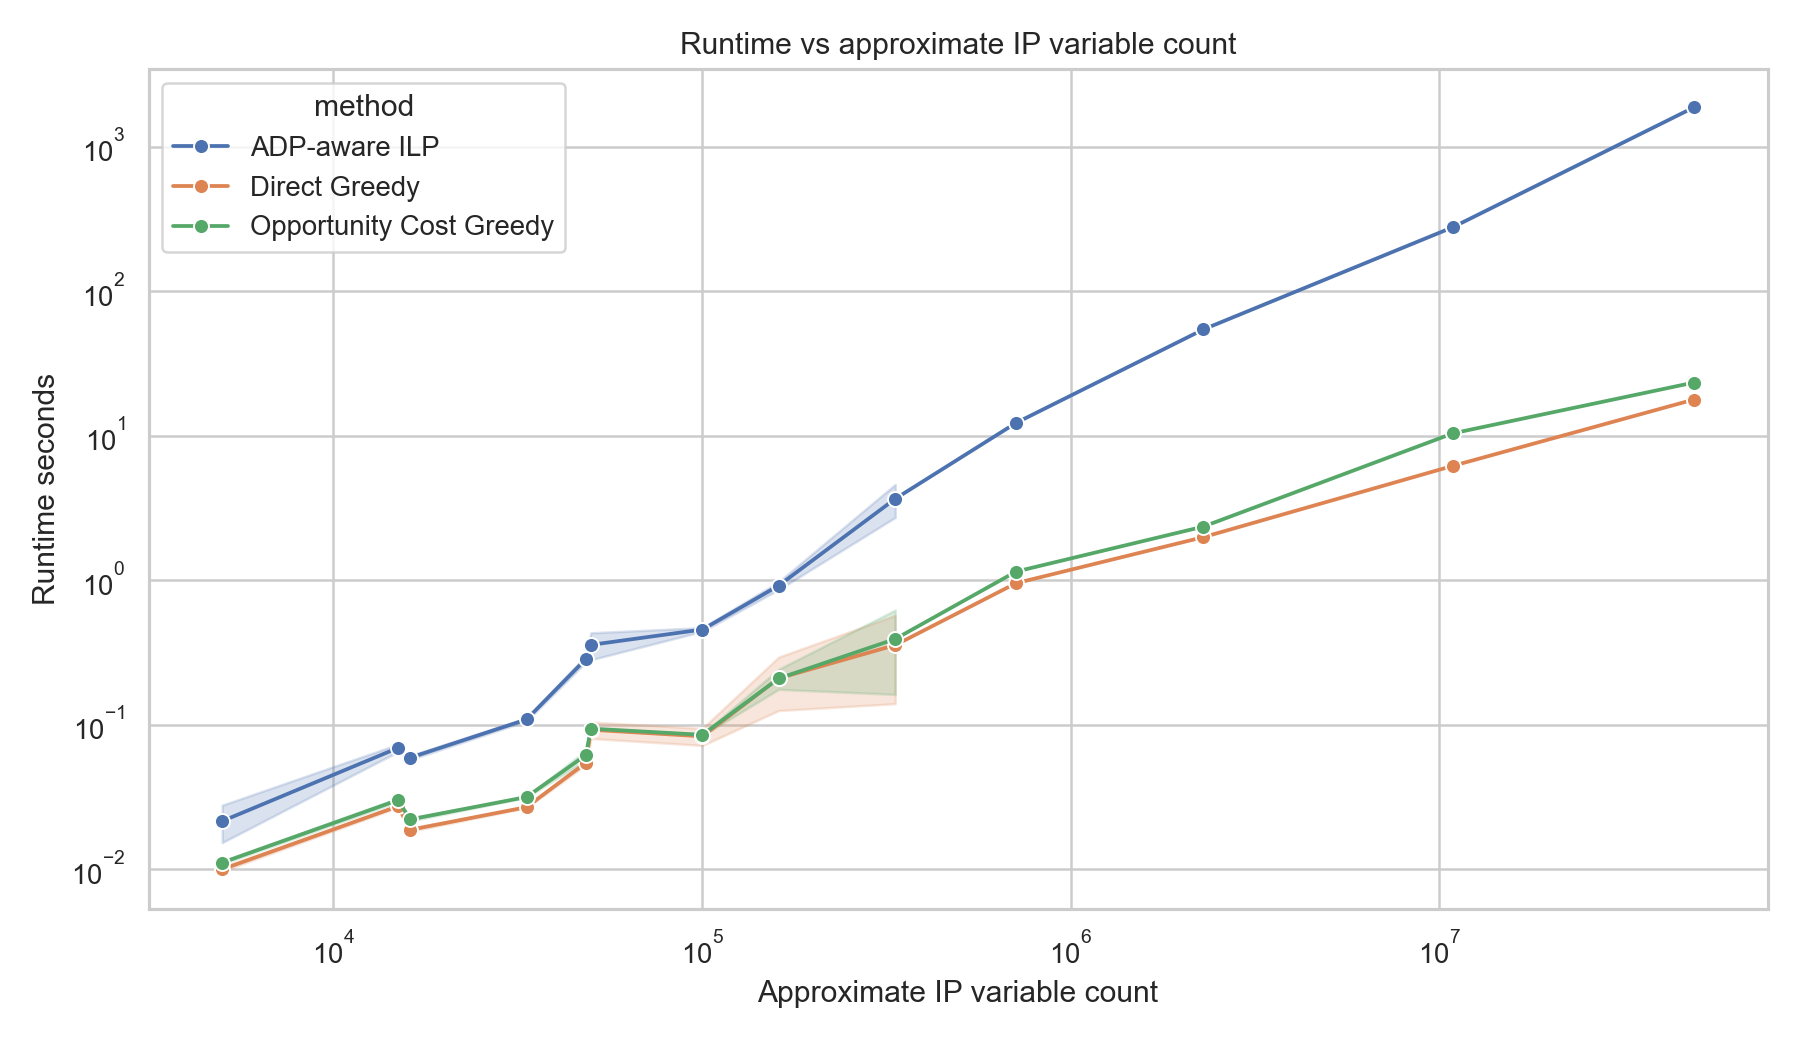
\includegraphics[width=0.88\linewidth]{experiments/synthetic/scaling_summary/runtime_by_variable_count.png}
  \caption{Runtime (seconds) versus approximate IP variable count for N6.}
\end{figure}

\subsection{Real-Data Validation}
To ensure practical applicability, we validated our algorithms on 2026 Yahoo and FanGraphs datasets (252 draft cases each). As shown in Table \ref{tab:real_data}, the ranking of the methods matches the synthetic findings perfectly. Opportunity Cost Greedy substantially reduces the optimality gap left by the naive Direct Greedy baseline on realistic draft settings.

\begin{table}[H]
\centering
\small
\caption{Real-data validation summary (Gap measured in absolute projected points).}
\label{tab:real_data}
\begin{tabular}{llrrr}
\toprule
Dataset & Method & Mean Objective & Mean Gap & Max Gap \\
\midrule
Yahoo 2026 & ADP-aware ILP & 7917.209 & 0.000 & 0.000 \\
Yahoo 2026 & Opportunity Cost Greedy & 7767.732 & 149.477 & 255.700 \\
Yahoo 2026 & Direct Greedy & 7662.866 & 254.343 & 373.000 \\
\midrule
FanGraphs 2026 & ADP-aware ILP & 14642.927 & 0.000 & 0.000 \\
FanGraphs 2026 & Opportunity Cost Greedy & 14320.135 & 322.792 & 508.000 \\
FanGraphs 2026 & Direct Greedy & 14097.337 & 545.590 & 644.500 \\
\bottomrule
\end{tabular}
\end{table}

\section{Conclusions}

This project successfully models fantasy baseball snake-draft planning as an operations research problem. The primary challenge was balancing positional constraints, market timing, and draft scarcity against the computational limits of exact optimization. 

Our empirical findings convey a clear message: while the ADP-aware ILP provides an undeniable exact benchmark, its exponential runtime growth renders it impractical for large-scale or real-time drafting applications. Our proposed method, \textbf{Opportunity Cost Greedy}, effectively solves this by estimating the delay-cost of waiting for future turns. Across all controlled synthetic environments—including elite-heavy distributions, rigid positional constraints, tight supply ratios, and highly noisy ADP markets—OCG consistently narrowed the optimality gap compared to the myopic Direct Greedy baseline. Furthermore, it proved its scalability by solving massive 50-million variable instances in seconds.

\textbf{Limitations and Future Work}: 
Currently, ADP serves only as a proxy for opponent behavior. In reality, human opponents do not follow ADP mechanically, and player projections carry inherent variance (e.g., injury risks). Future extensions could incorporate probabilistic opponent modeling, bench-value management, and hybrid methods that use OCG to generate an initial incumbent solution, followed by localized ILP repairs.

Overall, this project shows that while the ADP-aware ILP provides the exact benchmark for draft optimization, Opportunity Cost Greedy delivers a highly strategic, practical alternative that is fast enough to act as a real-time decision-support tool.

\end{document}